%!TEX root = root.tex
\label{sec:results_simulation}
\subsection*{Experimental setup}
%
%% \begin{figure}[t]
%%   \centering
%%   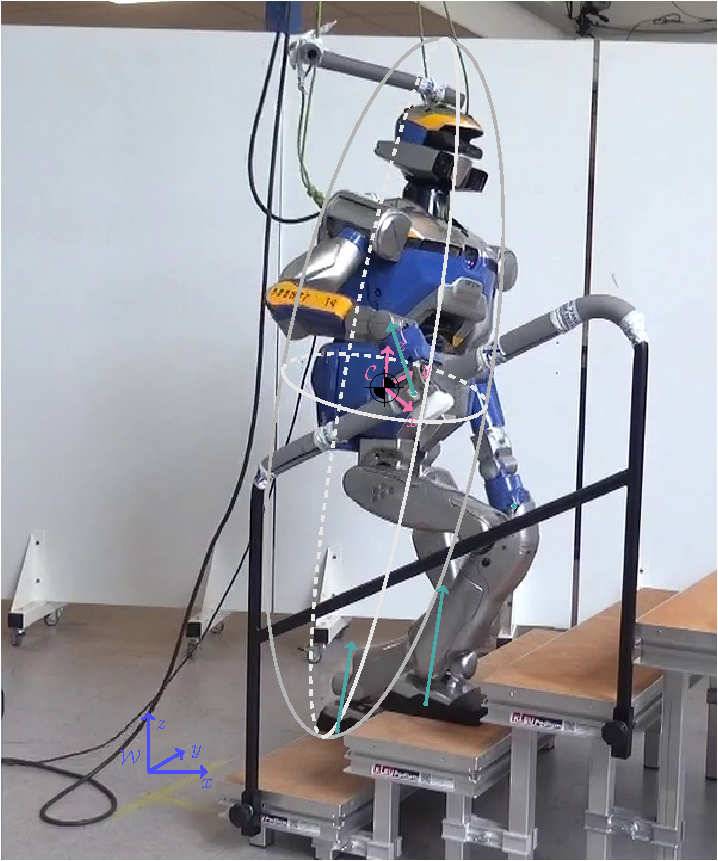
\includegraphics[width=1.0\linewidth, keepaspectratio]{%
%%       ./figures/tikz/reduced_model_setup_with_hrp2.pdf%
%%   }
%%   \caption{%
%%   Simulation of HRP-2 climbing stairs with support of a handrail using Pinnochio~\cite{pinocchio:laas}.
%%   The overlay shows the used reduced model (center of mass (CoM, black) at waist, CoM frame (magenta), gray inertia ellipsoid, contacts (teal dots) and contact contact forces (teal arrows) as well as world coordinate system $\mathcal W$ (blue).}
%%   \label{fig:openhrp_setup}
%% \end{figure}

We have considered the experimental setup depicted in Fig.\ref{fig:covermultimanuel} as proof-of-concept.
The goal is to make the humanoid robot HRP-2 climbing a stair case with a handrail as additional support.
The height, the depth, and the width of the stairs are respectively $15 cm$, $30 cm$, and $1 m$.
The hand rail is a cylinder with a diameter of $ 3 cm $.
% In an industrial environment, for example, the height of the stairs are irregular and the average height is around $ 20 cm $.
In this case the handrail is needed to avoid excessive power consumption in the leg motors.
\begin{figure}[ht]
%  \vspace*{0.3cm}
%  \begin{tikzpicture}
%  \node (MCS00) at (0,0) {\pgfuseimage{MCSET00png}};
%  \node (MCS01) at (2.5,0) {\pgfuseimage{MCSET01png}};
%  \node (MCS02) at (5,0) {\pgfuseimage{MCSET02png}};
%  \node (MCS03) at (7.5,0) {\pgfuseimage{MCSET03png}};
%  \node (MCS04) at (10,5) {\pgfuseimage{MCSET04png}};
%  \node (MCS05) at (12.5,5) {\pgfuseimage{MCSET05png}};
%  \node (MCS06) at (15,5) {\pgfuseimage{MCSET06png}};
%\end{tikzpicture}
\pgfuseimage{MCSET00png} \hfill
\pgfuseimage{MCSET01png} \hfill
\pgfuseimage{MCSET02png} \hfill
\pgfuseimage{MCSET03png} \\
\vspace*{-0.8cm}
\begin{center}
\pgfuseimage{MCSET04png} \hspace*{0.8cm}
\pgfuseimage{MCSET05png} \hspace*{0.8cm}
\pgfuseimage{MCSET06png}
\end{center}
    \caption{
        Set of contact stances realized by the humanoid robot HRP-2 using the method proposed in this chapter.
        The experiment has been realized 5 times in a row without failure.
        The accompanying video shows the realization of the experiments.
    }
\label{fig:contact_stances}
\end{figure}
%
Starting and ending in a half-sitting position of the robot, the motion is divided into $3$ phases that are executed twice:
(i) the right hand establishes contact with the handrail,
(ii) the right foot is set on top of the stair in front,
(iii) the left foot is lifted and placed next to the right one on the stair.
The robot is in double support phase during the movement of an end-effector and triple support phase during the CoM transition phase.
%The main difficulty is to to handle the latter.
%In case the contacts is not active, i.e. the limb is moving, the forces are set to $0$ in the $OCP$
See Fig.~\ref{fig:contact_stances} for snapshots of the real humanoid robot HRP-2 performing the motion.
%
% \begin{figure*}[h]
% \begin{center}
%         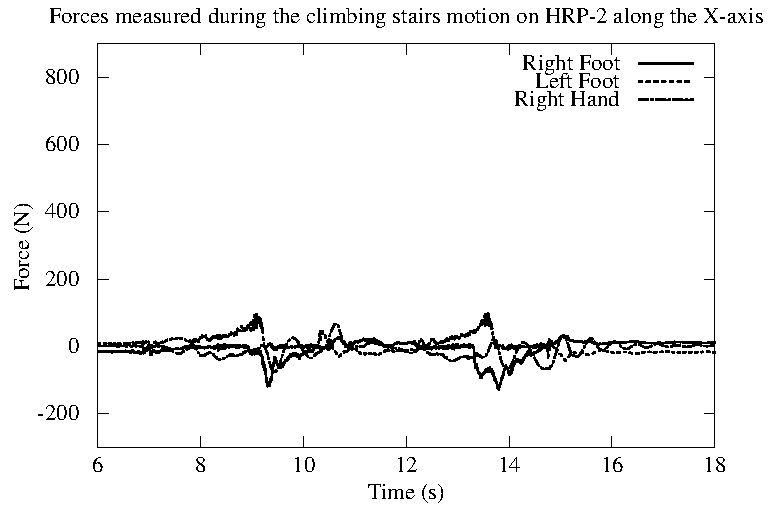
\includegraphics[width=0.3\linewidth, height=4.5cm ,keepaspectratio]{./figures/gcfx}
%         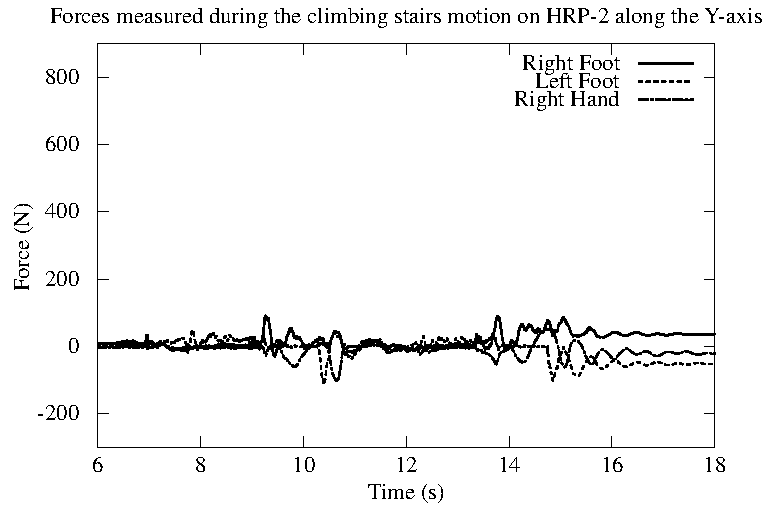
\includegraphics[width=0.3\linewidth, height=4.5cm ,keepaspectratio]{./figures/gcfy}
%         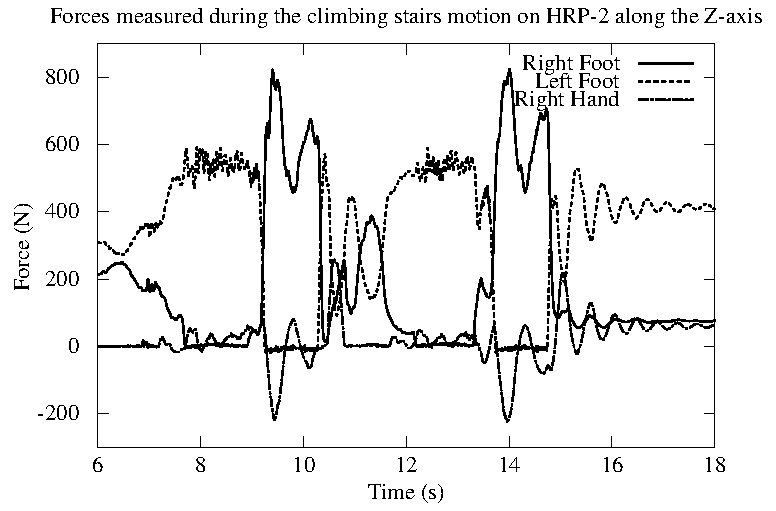
\includegraphics[width=0.3\linewidth, height=4.5cm ,keepaspectratio]{./figures/gcfz}
% \end{center}
%     \caption{%
%         Measured forces on the HRP-2 humanoid robot during the motion depicted in Fig.~\ref{fig:contact_stances}.
%         }
% \label{fig:measured_contact_forces}
% \end{figure*}
%

The robot moves an end-effector in $ 1.4 s $ and moves its center of mass position in $ 0.1 s $ during a transition phase.
The timing of the phase durations is crucial for the robot because they implicitly define the velocity of each limb.
From experience in ground-level walking, the period of single support and double support are usually around $0.7 s$ and $0.1 s$.
However, in this example the robot has to go through a larger distance at each phase than for ground-level walking.
Keeping the same schedule as in ground-level walking makes the robot reaching its actuators limits in speed and current more likely.

All the computations (contact planning and WPG) were performed offline.
A possible contact planner is open-source and available at \url{https://github.com/humanoid-path-planner}.
The OCP is solved using the proprietary software MUSCOD provided by the Interdisciplinary Center for Scientific Computing (IWR) of Heidelberg University.
This software offers a OCP toolkit (e.g. integration and numerical-differentiation routines) along with an efficient sparse sequential-quadratic-program solver.
In this experiment the solver condensed the problem before solving it.

The approach presented in this chapter has been developed to prove the concept of using a template model for a multi-contact controller.
In the control chain, only the OCP part is not yet run in real time.
In fact the computation time for the motion in the video attachment is $\sim30$ minutes.
The large computational foot print is due to
(i) calculating the motion all at once on the whole preview-window of $18.4 s$,
(ii) an over parametrization of the problem (3003 DoFs),
(iii) not exploiting the intrinsic sparsity resulting from the template model.
Future work will include a tailored implementation of the algorithm considering these bottlenecks and allow a real-time execution on the robot.
Despite this, the inverse dynamics run in $1 ms$ on the HRP-2 CPU ({\it Intel(R) Core2(TM) Duo $E7500$, frequency $2.8 GHz$, $1$ core, $3Mb$ of cache}) under Ubuntu 10.04 LTS.
%

\subsection*{Forces during contact transition}

Fig.~\ref{fig:measured_contact_forces} shows the forces measured during one experiment.
It appears that almost all the forces are acting along the $z$-axis.
The right hand has an important role as it can realize forces up to $200 N$ and more remarkably also exert negative forces at $9 s$ and $14 s$, i.e., the robot also pulls itself using the grip on the handrail.
Almost no torque is applied at the level of the feet, the propulsion of the robot is more visible in the tangential forces along the $x$- and $y$-axis.

Let us now focus on the $z$-axis.
At the beginning of the motion ,the robot is stable on its feet and no other contact with its environment is established (phase not shown in the graph).
At $6 s$ the hand comes into contact with the handrail causing perturbations in the feet force distribution.
The next transition appears just before $8 s$.
The robot shifts its CoM to the left foot and puts the right foot on the first stair.
Then the robot has three contacts with its environment and starts to use the hand contact.
It pushes with the right leg and pulls with the hand to climb the stair.
This particular motion excites the flexibility located under the ankle of HRP-2.
Between $10 s$ and $12 s$ the flexibility perturbs the system but the forces on the hand compensate for it.
The hand contact stabilizes the robot and allows it to move the hand towards the next grasping position at $12 s$, where the robot is back to a stable state again.
During the hand movement, the robot's CoM is affected by the flexibility exertion but not enough to fall down due the stabilizing influence of the grasping contact before and after the double support phase.
The motion is repeated once.
The only difference is that the hand does not release contact with the handrail at the end of the motion.
This helps the robot to stabilize and go back to an equilibrium state.
%
\begin{figure}[h]
  \centering
        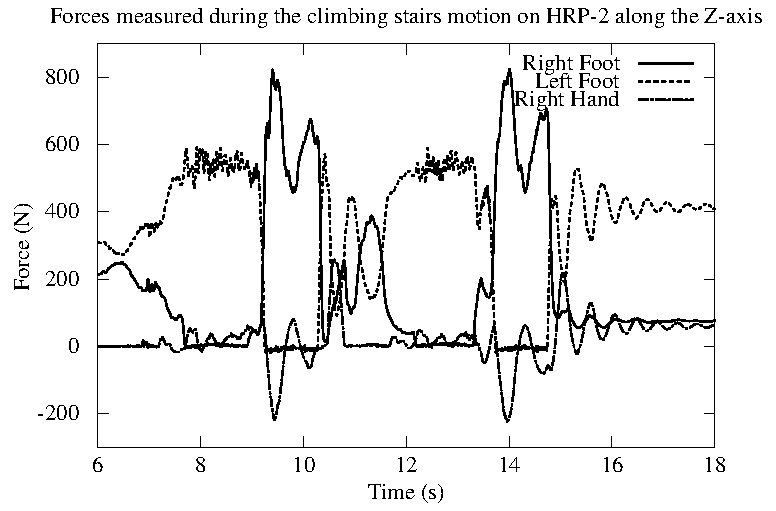
\includegraphics[width=0.35\linewidth, keepaspectratio]{./figures/gcfz.pdf} \\
        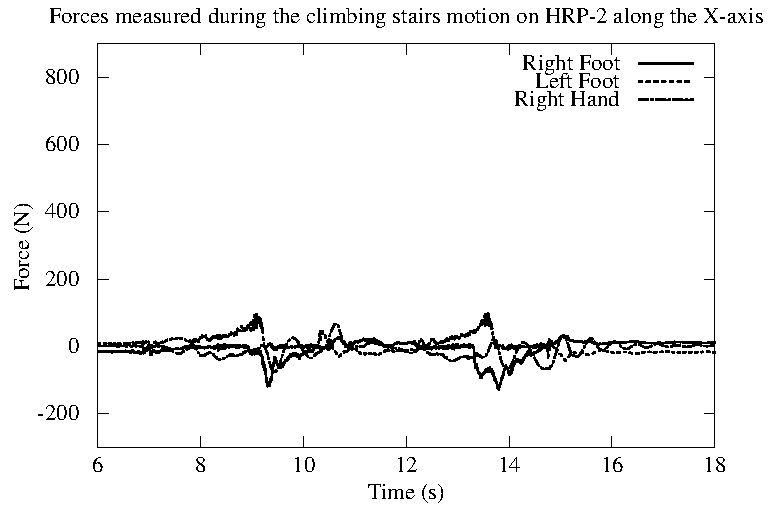
\includegraphics[width=0.35\linewidth, keepaspectratio]{./figures/gcfx.pdf}%
        %\hfill%
        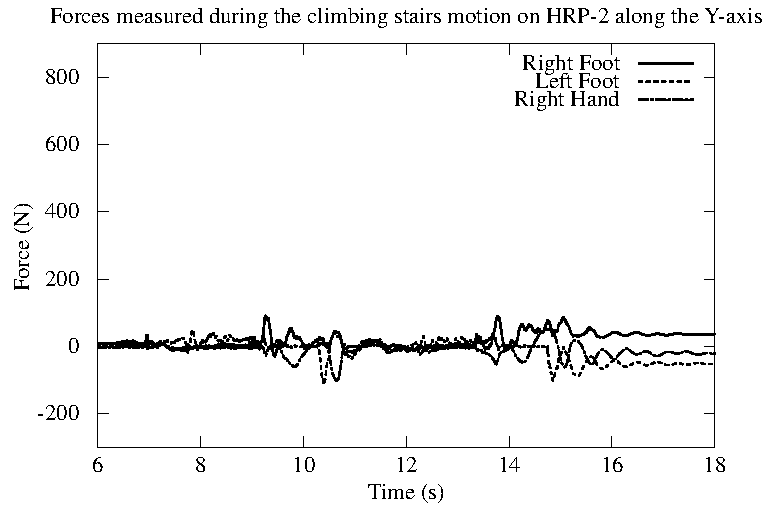
\includegraphics[width=0.35\linewidth, keepaspectratio]{./figures/gcfy.pdf}%
    \caption{%
        Measured forces on the HRP-2 humanoid robot during the motion depicted in Fig.~\ref{fig:contact_stances}.
        }
\label{fig:measured_contact_forces}
\end{figure}
%

\subsection*{Comparison between OCP and reality}

\begin{figure}[h]
  \centering
  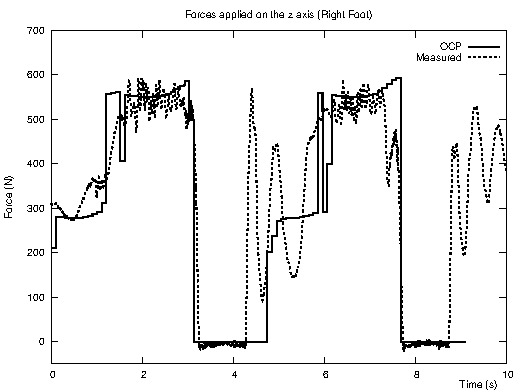
\includegraphics[width=0.35\linewidth , keepaspectratio]{./figures/forces_along_z_RF.pdf}\\%
  %\hfill%
  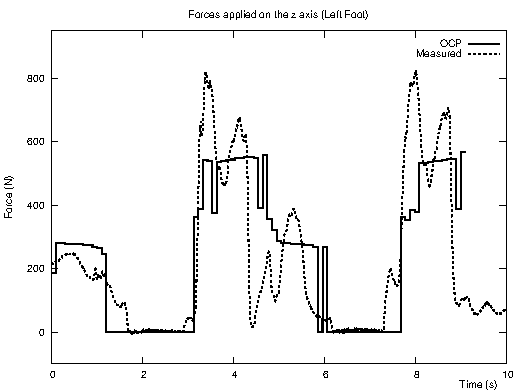
\includegraphics[width=0.35\linewidth , keepaspectratio]{./figures/forces_along_z_LF.pdf}%
  %\hfill%
  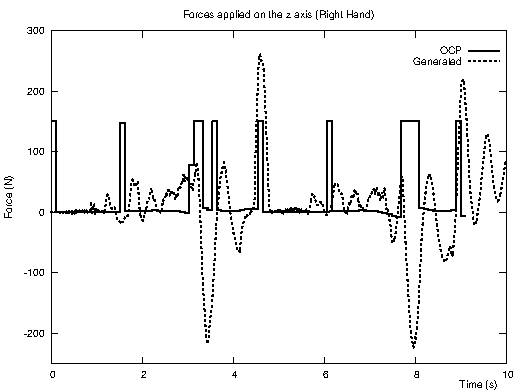
\includegraphics[width=0.35\linewidth , keepaspectratio]{./figures/forces_along_z_RH.pdf}
\caption{Measured forces on the HRP-2 humanoid robot during the motion depicted in Fig.~\ref{fig:contact_stances} compared with the OCP solution. The graphs present respectively the right foot, left foot, and right hand $z$ forces against time.}
\label{fig:measured_and_computed_forces}
\end{figure}

In Fig.~\ref{fig:measured_and_computed_forces} the measured $z$ forces are compared with the guessed ones from the OCP.
We can clearly see here that the two match at the beginning of the motion.
However the compliance placed under the HRP-2 ankle get excited when the robot lifts its weight from the ground to the first step.
This causes unplanned behavior as the flexibility is not modeled in the OCP.
As future work, we want to include a model of the flexibility inside the template model of the dynamics.


\subsection*{Current consumption}

\begin{figure}[h]
  \centering
    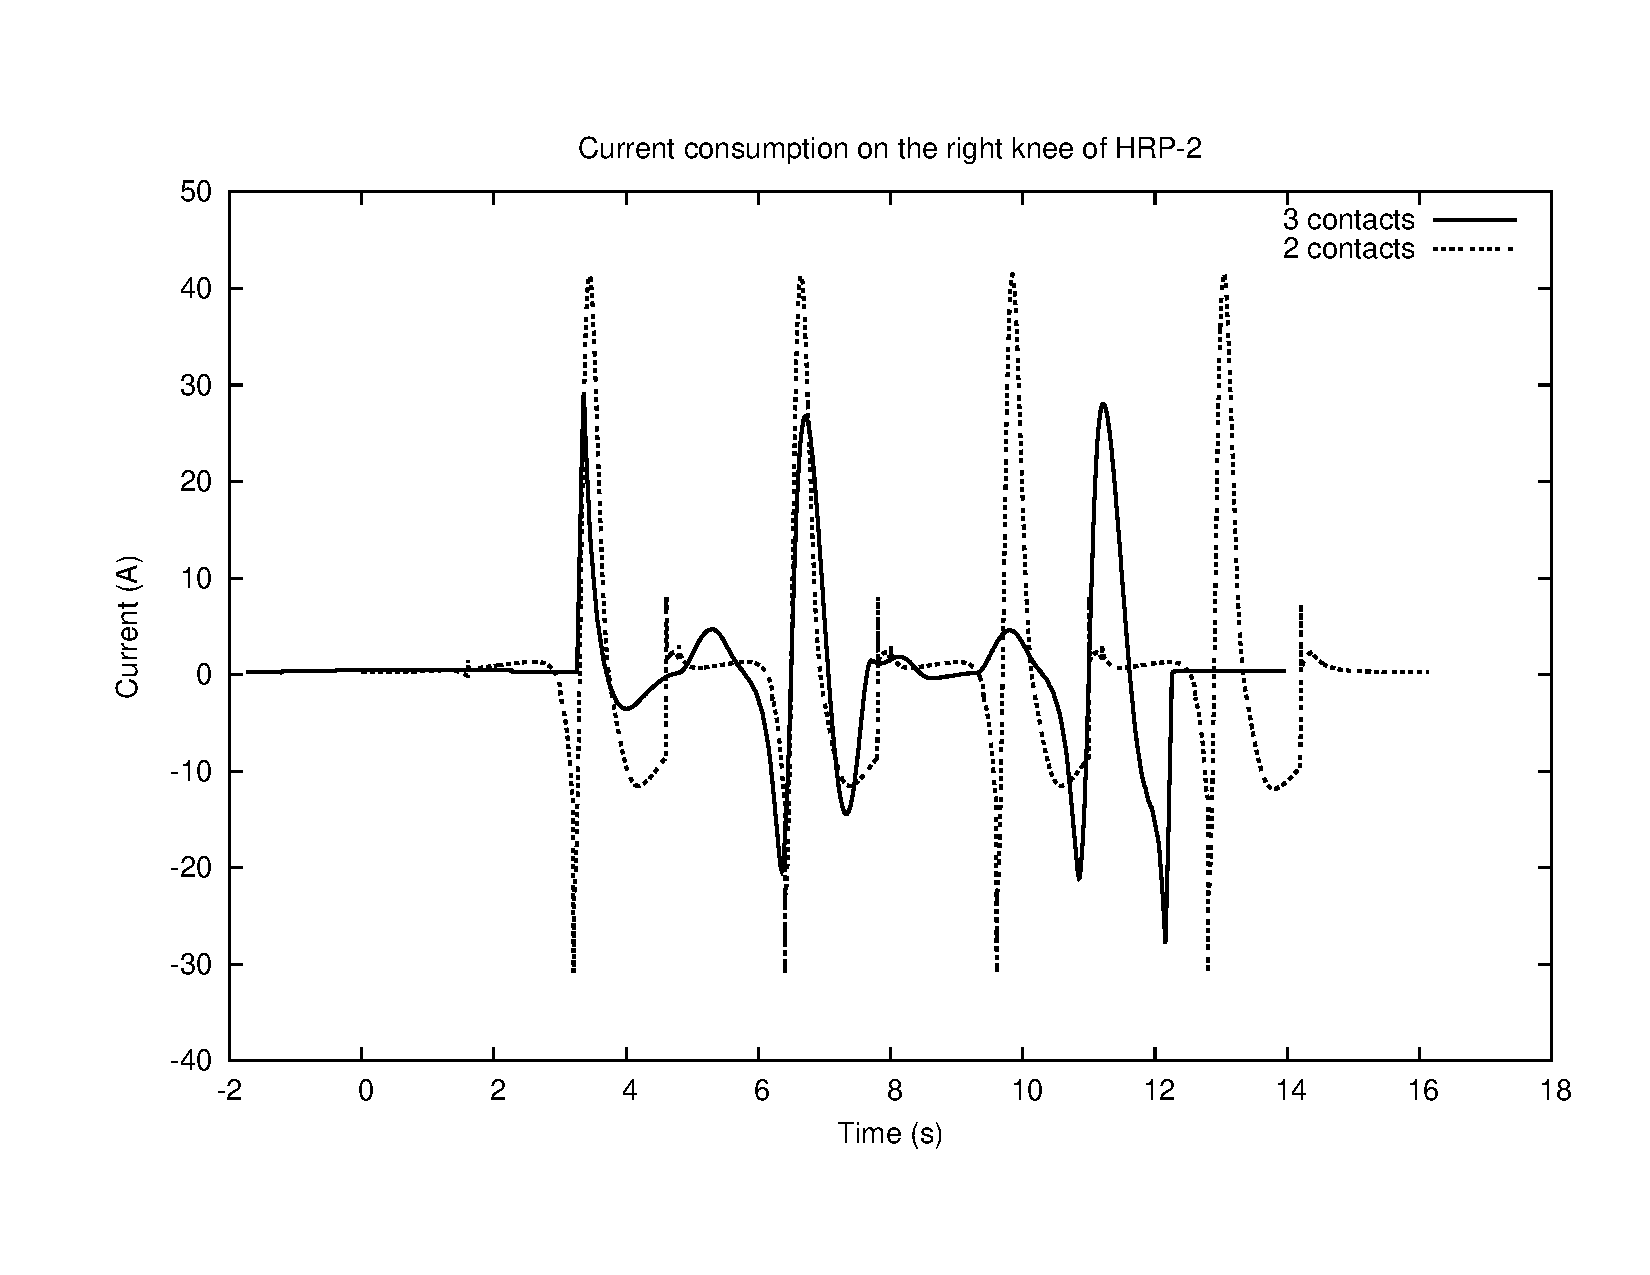
\includegraphics[width=0.35\linewidth]{./figures/RightKneeCurrent.pdf}
  \caption{Current consumption comparison between 2-contact locomotion and 3-contacts locomotion for climbing a 15 cm staircase.}%
  \label{fig:current_consumption}%
\end{figure}%

A severe limitation in climbing stairs with foot contacts only for human-sized humanoid robot is the current consumption.
After performing a large number of experiments on a $15 cm$ staircase using a different algorithm \cite{Morisawa:ICRA:2007}, it appears that the rate of success was highly dependent on the battery charge level.
Based on this observation, and using a model of the robot actuator, the maximum current amplitude was detected to be $40 A$ on the right knee as depicted in Fig.~\ref{fig:current_consumption}.
It is mostly due to the fact that the weight shifting is performed by one support leg.
Using several contact points during weight shifting allows to distribute the load across several actuators.
Therefore, the current asked for the right knee for the same motion using multiple contacts does not exceed $30 A$.
This allows to perform the motion depicted in Fig.~\ref{fig:contact_stances} 5 times in a row even with low battery charge level.

